\begin{savequote}[6cm]
<< What is this place

Filled with so many wonders?

Casting its spell

That I am now under >>

\qauthor{Fluttershy, So Many Wonders}
\end{savequote}

\chapter{DomVision : Application au réseau local domestique}
\chaptertoc
Nous avons présenté dans le chapitre d'introduction le contexte fil rouge sur lequel cette thèse s'appuie. Ce chapitre permet de mettre en pratique la solution d'observation. DomVision est l'instanciation d'Astronef-Asteroid sur le réseau local domestique. Ainsi, en quelques composants et en plusieurs requêtes, nous arrivons à mettre en œuvre un système d'observation.

Dans ce chapitre, nous présentons les différents points de mise en application qui nous permettent de valider notre contribution dans son ensemble. En premier lieu, dans la section~\ref{sec:valid:domvision:systeme}, nous présentons comment nous nous sommes adapté au système observé. Ensuite, en section~\ref{sec:valid:domvision:requetes}, nous détaillons les requêtes que nous avons pu déployer grâce à l'expressivité d'Astral. Cela couvre la mise à jour de la base de données comme les requêtes de l'utilisateur. Enfin, en section~\ref{sec:valid:domvision:architecture} nous démontrons la flexibilité de notre solution en introduisant un nouvel opérateur capable d'établir des préférences sur les observations.

\section{Adaptation au système observé}\label{sec:valid:domvision:systeme}
Dans cette section, nous analysons le système au sens où nous l'avons décrit jusqu'ici dans Astronef et Asteroid. Nous devons modéliser le système pour en extraire son schéma qui permettra de représenter le catalogue dans la base d'Asteroid. Puis nous nous intéressons aux données temps-réel. En enfin, nous présentons les flux à notre disposition dans ce réseau.

\subsection{Le schéma du système}
Nous présentons ici la vision que nous avons du système que nous observons. Il est important de voir que cette vision ne doit pas être lié aux sources de données disponibles. Elle a pour but de refléter l'interprétation de ou des experts souhaitant observer le système. Nous définissons ici 3 concepts principaux : les équipements, les applications et les interfaces réseaux.

\subsubsection{Équipements}
La notion d'équipement est une vision orienté utilisateur. En effet, un \textit{équipement} est un chassis physique. Les équipements virtuels ne sont ainsi pas représentés. Ce choix permet de représenter à l'utilisateur les appareils qu'il est capable de voir et de manipuler (débrancher par exemple). Quelques exemples : \textit{Livebox}, \textit{STB}\footnote{Set Top Box : Boitier connecté à une télévision pour fournir les services de partages de contenus, de télévisions, VOD...}, Ordinateurs, Tablettes, Disques durs réseaux.

Un équipement \textit{peut} avoir un \textit{numéro de série} unique. Cela représente a priori son seul moyen d'identification. Mais d'autres heuristiques peuvent être faites avec les autres concepts.

\subsubsection{Applications}
Nous désignons par \textit{application} un programme instancié sur un des équipements. À un \textit{équipement} est associé plusieurs \textit{applications}. Les \textit{applications} permettent d'effectuer des tâches sur leurs équipements respectifs. Une \textit{application} en exécution est considéré comme \textit{active} ou à l'inverse \textit{inactive}. Quelques exemples : Partage de contenu, Agent d'administration, Gestion d'impression.

Une \textit{application} a un \textit{nom}, une \textit{description} textuelle et potentiellement un \textit{type}. Il est nécessaire de pouvoir identifier une application pour un équipement donné par son \textit{nom}, l'unicité sur son \textit{type} ou si disponible un identifiant de processus.

\subsubsection{Interfaces réseaux}
Les \textit{interfaces réseaux} sont moins sujets à interprétation que les deux concepts précédents. Une \textit{interface réseau} représente un moyen de connexion que possède un \textit{équipement}. Nous supposons que cette interface est une interface \textit{MAC}\footnote{Permettant des interfaces \textit{IP} et \textit{Zigbee} potentiellement}. Elle possède un \textit{nom} système unique pour l'équipement, un type (wifi, ethernet), ainsi qu'une adresse \textit{MAC} considéré unique sur le réseau et d'autres adresses comme \textit{IPv4} ou \textit{v6}.

L'identification de ces interfaces peut être faite via ses adresses, bien que seule l'adresse \textit{MAC} garantisse l'unicité.

\subsubsection{Concepts supplémentaires possibles}
Ayant une modélisation des concepts principaux du réseau local domestique, nous pouvons maintenant ajouter des concepts supplémentaires. Bien que nous ne les utiliserons pas dans la suite de ce chapitre, il est intéressant d'en voir quelques exemples.

Les \textit{services} sont des compositions d'\textit{applications}. Ils permettent de fournir des expériences à l'utilisateur de plus haut niveau. À ces \textit{services}, nous pouvons attacher des contrats de services.

Enfin, pour développer la topologie du réseau, les \textit{liens} relient deux interfaces réseaux. Les \textit{chemins} composent des \textit{liens} réseaux. Et les \textit{canaux de transport} peuvent utiliser un \textit{chemin} pour aussi relier deux \textit{applications}. Toutefois, la collecte de ces informations est soumise à des contraintes de mise en œuvre plus technique comme l'utilisation de protocoles \textit{LLTD} ou \textit{IEEE 1905.1}.

\subsection{Les données volatiles intéressantes}
Les données \textit{volatiles} sont les données temps-réel que nous souhaitons archiver en vue d'une analyse a posteriori. En premier lieu, nous explorons les historiques de métriques. Ces données sont en général utilisées sur des graphiques afin de détecter des comportements anormaux.

Les métriques de charge seront pour nous les données à surveiller. En effet, la surveillance de la santé du réseau local passe avant tout par la surveillance de ses paramètres reflétant sa charge. Pour les équipements, nous surveillons la charge processeur utilisé (en \%) et mémoire occupée (en ko). Pour les interfaces réseaux, le débit est un bon indicateur de sa saturation. Toutefois, même si la donnée est difficile à obtenir, la capacité maximale de l'interface permet de savoir la charge totale de l'interface. Si nécessaire, d'autres métriques plus spécifiques pourront être enregistrées, par exemple : la latence ou la gigue d'une interface réseau .

Nous souhaitons aussi être capable de traquer les changements de structure du réseau réseau local. Pour cela, nous pouvons surveiller et historiser les changements d'adresse \textit{IP} des interfaces, ou de statut (actif/inactif) des équipements, applications et interfaces.

Avec ces données combinées avec les capacités d'interrogations que nous avons, nous devons être capable de surveiller le réseau local domestique et si nécessaire aider l'établissement de diagnostiques.

\subsection{Les données disponibles}
Dans notre mise en œuvre, nous utilisons le protocole \textit{UPnP} largement répandu dans le réseau local actuellement. Ce protocole permet d'annoncer un \textit{Device}\footnote{Attention au vocabulaire utilisé par le protocole. Un \textit{device} UPnP est en réalité une \textit{application} déployée sur un \textit{équipement}.} sur le réseau. Ce \textit{Device} expose des \textit{Services} qui contiennent des \textit{Actions} qu'il est possible d'invoquer à distance. Les \textit{Devices} répondent à des profils la plupart du temps standards.

L'annonce des \textit{Device} \textit{UPnP} sur le réseau produit un flux de donnée \begin{center}\textit{UPnPStatus}(uuid, ip, type, friendlyName, status, $\t$).\end{center} Ce flux indique que le \textit{device} exposé avec l'IP \textit{ip}, ayant pour identifiant unique \textit{uuid}, pour profil \textit{type} et pour description textuelle \textit{friendlyName} a changé son statut au temps $\t$ pour \textit{status} (\textit{active}/\textit{inactive}).

Nous avions exploré en section~\ref{sec:rw:supervision:administration} que les protocoles et agents d'administrations pouvaient être de bons interlocuteurs pour fournir des données. Dans le monde \textit{UPnP}, il existe le profil \textit{DeviceManagement} capable de fournir des données intéressantes. Toutefois, ce profil n'est pas déployé sur tous les équipements. Le tableau~\ref{tab:valid:domvision:upnpdm} indique les données que nous exploitons. Les flux produits auront en plus des paramètres les attributs \textit{uuid} correspondant à l'identifiant \textit{UPnP} de l'agent, ainsi que le \textit{timestamp} d'émission $\t$.

\begin{table}
\centering
\begin{tabular}{|m{0.25\textwidth}|>{\ttfamily}m{0.25\textwidth}|m{.4\textwidth}|} \bottomrule
\rowcolor{hypcolor} Nom du flux & \rm Paramètre & Description du paramètre\\ \hline
\multicolumn{3}{|c|}{/UPnP/DM/DeviceInfo/PhysicalDevice/} \\\hline
Serial & {SerialNumber} & Numéro de série de l'équipement\\\hline
\multirow{3}{*}{NetworkInterface} & {SystemName} & Nom de l'interface réseau\\\cline{2-3}
& {MACAddress} & Adresse MAC de l'interface\\\cline{2-3}
& InterfaceType & Type de l'interface \\\hline
\multicolumn{3}{|c|}{/UPnP/DM/Configuration/} \\\hline
\multirow{2}{*}{IPInterface} & SystemName & Nom de l'interface réseau \\\cline{2-3}
& IPv4Address & Adresse \textit{IPv4} de l'interface \\ \hline
\multicolumn{3}{|c|}{/UPnP/DM/Monitoring/} \\\hline
\multirow{2}{*}{OperatingSystem} & CPUUsage & Charge actuelle du processeur\\\cline{2-3}
& MemoryUsage & Charge actuelle de la mémoire\\ \hline
\multirow{3}{*}{IPUsage} & SystemName & Nom de l'interface réseau\\ \cline{2-3}
& TotalBytesSent & Nombre d'octets envoyés \\\cline{2-3}
& TotalBytesReceived & Nombre d'octets reçus \\ \toprule
\end{tabular}
\caption{Listes des flux intéressant fournis par le profil UPnP-DM}\label{tab:valid:domvision:upnpdm}
\end{table}

\subsection{Les sources Astronef}
Nous avons conçu un composant spécifique pour la formation du flux \textit{UPnPStatus}. Ce composant n'a pas de paramètre et fournit directement l'interface \textit{Source} avec comme attributs ceux mentionnés. Son fonctionnement est événementiel.

Pour la communication sur \textit{UPnP-DM}, nous souhaitons un profil plus réutilisable. Nous avons conçu un composant générique capable d'interroger tous les nœuds de l'arbre et de fonctionner de manière événementielle et périodique. Le mécanisme d'événement ne provient pas du protocole car les paramètres que nous souhaitons observer ne sont pas en \textit{EventOnChange} (production d'une notification en cas de changement). Concernant l'accès à la donnée, le composant devra itérer si nécessaire pour récupérer toutes les instances (\#) d'un chemin et enverra l'ensemble des données dans un seul \textit{batch}. L'ensemble des paramètres de cette source est présenté dans la table~\ref{tab:valid:domvision:dmsource}.

\begin{table}[ht]
    \centering
    \begin{tabular}{cl}
        paramètre & description \\ \midrule
        path & Chemin d'accès aux données \\
        parameters & Liste CSV des paramètres souhaités \\
        period & Période de mise à jour du flux (optionnel) \\
        channel & Canal interne d'événement à souscrire (optionnel)
    \end{tabular}
    \caption{Paramètres du composant \textit{DMSource}}\label{tab:valid:domvision:dmsource}
\end{table}

Ainsi, pour les flux \textit{OperatingSystem} et \textit{IPUsage}, nous y accéderons périodiquement, et pour les autres, ils seront récupérés à chaque arrivée de \textit{Device} de ce profil\footnote{Nous aurions aussi pu faire une représentation à base de manipulation temporelle comme dans Asteroid.}. Pour cela, nous formons la requête $\sigma_{status=active\wedge type=dm}$ \textit{UPnPStatus}. Cette requête sera injecté dans le puit \textit{SourceNotifier} dont le but est de notifier les \textit{Sources} s'étant inscrit dans un canal d'événement. Ici, toutes les instances de \textit{DMSource} souhaitant être notifiées le seront dans le canal \textit{DM}.

Nous avons vu la représentation du système, les données intéressantes, et comment obtenir ces données. Nous présentons désormais des exemples de requêtes que nous posons au système d'observation pour démontrer son expressivité.
\section{Expressivité du système d'observation}\label{sec:valid:domvision:requetes}
\subsection{Entretien du modèle descriptif}
\subsection{Historisation des paramètres}
\subsection{Formations d'alertes}
\section{De l'algèbre aux composants}\label{sec:contrib:astronef:architecture}
Dans cette section, nous détaillons les éléments d'architectures que nous avons mis en œuvre pour permettre à une requête Astral d'être instanciée en un processus de traitement. Nous abordons premièrement les principes architecturaux utilisés. Ensuite, nous détaillons les différents composants utilisés dans Astronef. Enfin, nous présentons notre méthode extensible de construction de plan par l'utilisation d'un système de règles.
\subsection{Architecture}
Avant de détailler l'architecture de notre système de traitement de requêtes continues, nous allons d'abord présenter le paradigme architectural dans lequel nous allons mettre en œuvre Astronef. Nous présentons premièrement et brièvement les architectures à services. Puis, nous détaillons les principes des architectures à composants orientés services que nous utilisons par la suite.
\subsubsection{Architecture à service}
Les architectures à services permettent aux applications d'être assemblés sous forme de blocs réutilisables étant des \textit{services}. Un \textit{service} est définit par une spécification (ou \textit{description}, ou \textit{contrat}), qui décrit sa syntaxe, son comportement, sa sémantique ainsi que sa dépendance aux autres services. Dans les architectures à service, les services interagissent via un patron récurrent d'interaction (fig~\ref{fig:contrib:astronef:services}). 
\begin{figure}[ht]
    \centering
    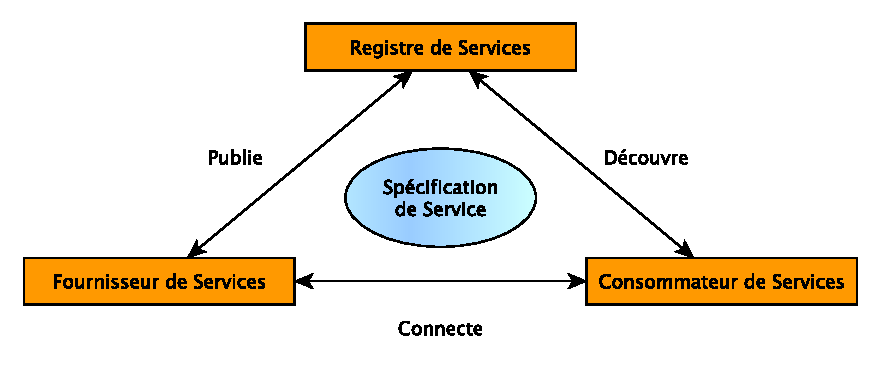
\includegraphics[width=0.7\textwidth]{contrib-astronef-services}
    \caption{Patron d'interaction de service}\label{fig:contrib:astronef:services}
\end{figure}
Un fournisseur de service va publier sa spécification à un registre. Un consommateur de service découvre le service fournit par une requête sur le registre. Enfin, le consommateur et le fournisseur se connectent. Le point clé de cette architecture étant que cette résolution est faite au \textit{runtime}.

\subsubsection{Architecture à composants orientés services}
Le modèle d'architecture à composants orientés services~\cite{Cervantes:servicecomponent} permet la mise en œuvre d'applications à base de services dans le paradigme de la programmation par composants. Le principe étant de séparer les mécanismes des architectures à services du code implémentant le comportement du service fournit. Ainsi, voici les principes d'un tel modèle :
\begin{itemize}
    \item Un service est une fonctionnalité fournie.
    \item Un service est caractérisé par sa spécification.
    \item Les composants implémentent des spécifications de services, qui peuvent eux-mêmes dépendre, du fait de leurs implémentations, d'autres services.
    \item Les patrons d'interactions de services sont utilisés pour résoudre les dépendances de services au \textit{runtime}.
    \item Les compositions sont décrites en terme de spécifications de services.
    \item Tout composant peut se substituer par un autre si les spécifications de services sont identiques.
\end{itemize}
Nous mêlons donc dans un même modèle, les idées de composants et de services. De plus, en s'inspirant des modèles récents tels que Fractal~\cite{Bruneton:fractal}, chaque composant possède un ensemble de propriétés (ou attributs) configurables. Nous obtenons aussi le pouvoir d'instancier (grâce aux fabriques) des composants à partir de configurations.

\begin{figure}[ht]
    \centering
    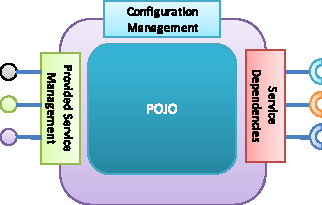
\includegraphics[width=0.5\textwidth]{contrib-astronef-ipojo}
    \caption{Un composant iPojo}\label{fig:contrib:astronef:ipojo}
\end{figure}
La figure~\ref{fig:contrib:astronef:ipojo} représente un composant dans l'implémentation \textit{iPojo}~\cite{Escoffier:ipojo}. Le principe étant que le code du composant (le \textit{POJO}, \textit{Plain Old Java Object}) est embarqué dans un conténaire auxquels seront accrochés des gestionnaires. Les trois couramment utilisés sont les gestionnaires de dépendances, de production de service, et de configuration. Ainsi, un composant pourra s'exposer sur un registre, tout en dépendant d'autres services et en supportant le fait d'être configurable.

\subsection{Les différents composants et services}
L'architecture d'Astronef est entièrement dirigé par ces approches. De multiples composants sont ainsi créés et instantiables, pour former une requête. Afin de pouvoir exécuter les requêtes, nous définissons trois services centraux :
\begin{itemize}
	\item[\textbf{Les \textit{EventProcessor}}] : Ces services ont deux primitives, l'une exécute une tâche quelconque, l'autre indique les autres \textit{EventProcessors} dont il dépend.
	\item[\textbf{Le \textit{Scheduler}}] : Ce service permet la planification. Ses primitives permettent aux différents \textit{EventProcessor} d'exprimer leur volonté de s'exécuter. Ce service devra mettre en ordre ces demandes en fonction des dépendances exprimés.
	\item[\textbf{Le \textit{QueryRuntime}}] : Ce service permet d'exécuter une requête. Il est lié à un \textit{Scheduler}, et utilise la primitive \textit{next} de celui-ci pour connaître la prochaine tâche qu'il faudra exécuter.
\end{itemize}

Nous adoptons ainsi l'approche émise par~\cite{Carney:scheduling} pour gérer l'ordonnancement des événements. Maintenant que nous avons vu les différents services nécessaire à l'exécution. Nous avons plusieurs types de composants que nous pourrons instantier :
\begin{itemize}
	\item[\textbf{Les entités}] : Fournissent les services nécessaires pour manipuler un flux ou une relation. Ces entités servent de résultats intermédiaires (ou de tampons). De plus, ils permettent un service de notification. En cas de changement, les \textit{EventProcessor} abonnés seront notifiés. Ainsi, ces composants nécessitent un \textit{Scheduler} pour demander l'exécution de leurs abonnés.
	\item[\textbf{Les sources}] : Une source nécessite une entité en lecture, dont elle manipulera le contenu pour la remplir. Ce composant pourra nécessiter le \textit{Scheduler} pour, entre autres, notifier la fin de son envoi et donc la fin de la requête.
	\item[\textbf{Les opérateurs}] : Nécessitent $n$ entités en lecture, et une autre particulière en écriture. Ce composant doit fournir le service \textit{EventProcessor}. Les implémentations des opérateurs bloquants pourront faire appel au \textit{Scheduler} pour planifier des exécutions ponctuelles.
	\item[\textbf{Les puits}] : Nécessitent une entité en lecture. Ce composant fournit le service \textit{EventProcessor} et doit être non-bloquant (donc seulement s'abonner à son entité en lecture).
\end{itemize}

Ainsi pour créer une requête : l'utilisateur doit fournir un ou plusieurs composants sources et un composant puit. Par la suite, il demande à Astronef de lui instantier ses sources et son puit en configurant les composants selon sa volonté. Enfin, il spécifie l'expression algébrique liant les sources au puit.

\subsubsection{De l'importance de la réutilisation}
Le fait d'abstraire l'architecture d'\textit{Astronef} permet une grande flexibilité architecturale. Tout d'abord, pour chaque composant, le fait de pouvoir le configurer tout en gérant son cycle de vie permet de réutiliser le même module pour plusieurs usages. Par exemple, supposons l'existance d'une source capable de récupérer une information périodiquement sur un protocole donné. Cette source pourra être utilisé pour plusieurs requêtes sous différentes instances en ayant plusieurs configurations.

Mais cette abstraction sous forme de services permet surtout la substitution. En effet, nous pouvons remplacer n'importe quel composant du moment qu'il supporte le même service. Nous utilisons ce principe pour sélectionner les meilleurs composants pour remplir le plus efficacement leurs rôles. De plus, l'utilisateur peut apporter ses propres implémentations pour étendre les capacités de l'intergiciel.

\subsection{Construction du plan par règles}
Nous définissons un plan de requête comme un ensemble de composants déployés pour répondre à la requête de l'utilisateur. Nous souhaitons avant tout que l'utilisateur n'ai pas à intervenir lors de cette construction. De son point de vue, il ne doit écrire que l'expression algébrique de sa requête et il doit être garanti d'une mise en œuvre efficace.

Pour atteindre ce but, nous avons choisi de mettre en place un moteur de règle. Le principe étant que nous partons de l'expression algébrique, puis nous itérons suivant plusieurs schéma d'inférences jusqu'à obtenir un plan de requête. Nous remarquons plusieurs avantage à une telle approche :
\begin{itemize}
	\item Intégration naturelle des connaissances. L'algèbre est pleine de propriété et de théorèmes. Il est nécessaire de pouvoir les exprimer dans un langage déclaratif pour les exploiter et pour en rajouter le plus possible.
	\item Expression de la sémantique des composants par l'algèbre. Comme il est nécessaire d'associer des composants logiciels à la sémantique d'Astral, il est nécessaire de spécifier à quelle opération chaque composant (et chaque paramètre de configuration) répond. Cela permet une clarification des sémantiques d'exécution.
	\item Extensibilité très forte. En considérant que l'ajout de nouveaux composants peut se faire via l'ajout de nouvelles règles, il devient aisé d'étendre le système pour permettre des opérateurs, ou des optimisations qui n'étaient pas prévues.
\end{itemize}

Afin de mettre en œuvre cet ensemble de règle pour obtenir un plan de requête efficace, nous faisons une analogie avec les systèmes de gestions de base de données. Comme présenté dans la section~\ref{sec:rw:sgfd:optim}, l'optimisation est découpé en deux parties : l'optimisation logique, et l'optimisation physique. Nous réutiliserons cette approche qui a fait ses preuves au fur et à mesure des années. Nous restructurerons donc la structure de l'expression algébrique dans la section~\ref{sec:contrib:astronef:logique} pour qu'elle soit plus optimisé. Ensuite, nous sélectionnerons les meilleurs composants et les meilleures configurations pour mettre en œuvre cette nouvelle expression, dans la section~\ref{sec:contrib:astronef:physique}.

Nous utilisons un moteur capable d'exécuter du Prolog~\footnote{En réalité, le langage utilisé (PROVA~\cite{Kozlenkov:prova}) est un dérivé de Prolog mieux adapté à l'intégration avec Java. Mais le principe reste tout à fait similaire.}, langage de programmation logique, pour appliquer nos règles. Avant de détailler l'ensemble de ces règles, nous présentons d'abord la structure d'une expression. Toute expression étant structuré sous forme d'arbre, il est possible de représenter une requête avec des nœuds de la forme\footnote{L'utilisation d'objets de propriétés fait partie du langage PROVA, mais cela reste formalisable en Prolog standard avec une liste d'éléments [clé,valeur].} :
\begin{center} [$\underbrace{A}_{\textrm{Nature du nœud}}$, $\underbrace{B}_{\textrm{Ensemble de propriétés}}$, $\underbrace{C}_{\textrm{Liste de nœuds fils}}$] \end{center}
\begin{example}
	Soit $R$ une source déclaré dans le système, nous souhaitons exécuter la requête $\sigma_{id=1} R$. Alors l'expression de cette requête est la suivante :
	\begin{lstlisting}
[sigma,	{"condition":"id=1"}, [
	[source, {id:"R"}, []]
]]
	\end{lstlisting}
\end{example}
Nous remarquons que cette syntaxe est très similaire au \textit{XML}, c'est pour cela que ce langage est celui utilisé en pratique pour spécifier des requêtes dans le prototype. Il est ensuite traduit en expression utilisable en Prolog. L'ensemble des nœuds possibles corresponds aux différents opérateurs de l'algèbre. Nous ne détaillerons pas ceci dans ce manuscrit. Le lecteur pourra consulter le manuel sur la page web suivante \url{http://code.google.com/p/astral/wiki/XMLSyntax} pour trouver les expressions exactes supportées.
\section{Conclusion}
Ce chapitre a dressé un état de l'art des différents systèmes capables d'offrir une solution générique de supervision. Il en ressort qu'aucun système ne supporte entièrement les critères de qualité que nous nous sommes fixés. Le tableau~\ref{tab:rw:supervision:bilan} résume les 11 points d'analyse en colorant les différentes points suivant leurs conformités. 

\begin{sidewaystable}[ht]
\centering
\begin{tabular}{@{{\vrule width 1pt}\ \ }>{\raggedleft}m{3cm}@{\ \ {\vrule width 1pt}\ \ }M{4.2cm}|M{4.2cm}|M{4.2cm}|M{4.2cm}@{\ \ {\vrule width 1pt}}} \bottomrule
\head Critère & \head Système d'administration & \head Gestion de contexte & \head Entrepôts de données & \head Gestion de flux de données \\  \toprule \bottomrule
\critereAA & Hiérarchique & Triplets & Relationnel & Relationnel dérivé \\ \hline
\critereAB & \meh Structure hiérarchique sans contraintes & \good Ontologies & \good Modèle relationnel normalisé & \bad Pas de structure \\ \hline
\critereAC & \meh Notifications & \bad Ajout du temps en propriété & \meh CDC & \good Flux natif \\ \toprule \bottomrule
\critereBA & \meh Instantanée, continu en ad-hoc & \bad Instantané principalement & \meh Instantané. ETL en pseudo-continu & \bad Continu uniquement \\ \hline
\critereBB & \good Standardisation, union de modèles & \meh Fusion d'ontologies non standardes & \good Processus ETL (complexe) & \good Union et jointures de flux \\ \hline
\critereBC & \bad Impératif principalement & \good Logique & \meh Déclaratif (SQL) et Procédural (ETL) & \good Déclaratif principalement\\ \hline
\critereBD & \meh Procédures à écrire soi-même & \good Logique du premier ordre & \good Relationnel multidimensionnel et Algorithmie dédiée & \meh Relationnel avec support du dynamisme\\ \toprule \bottomrule
\critereCA & \good Support des standards & \meh Spécification longue des domaines & \bad Spécification du schéma, des ETL, autre (complexe) & \good Écriture de requêtes \\ \hline
\critereCB & \bad Aucune & \good Séparation par les domaines & \good Données multidimensionnelles & \bad Aucune \\ \hline
\critereCC & \good Modèle extensible, fonctions métiers dans le gestionnaire & \meh Capteurs virtuels & \good Opérateurs ETL, procédures SQL, algorithmes & \meh Sources et puits mais pas les opérateurs  \\ \hline
\critereCD & \good Large échelle & \bad Complexité très haute & \meh Réactivité lente, Support de grande quantité & \good Support de haut débits\\ \toprule 
\end{tabular}
\caption{Récapitulatif de l'état de l'art des systèmes génériques de supervision}\label{tab:rw:supervision:bilan}
\end{sidewaystable}
Il en ressort que les systèmes d'administrations sont avant tout des systèmes qui fonctionnent grâce au support des standards et à leur simplicité d'implémentation. L'architecture avec gestionnaire adaptable grâce à des langages impératifs permets une grande flexibilité pour s'adapter aux cas d'usages. De son côté, l'informatique contextuelle fournit des outils permettant de modéliser et manipuler proprement les concepts du système grâce aux ontologies et aux raisonnements logiques. Il en sort une claire séparation des domaines de compétences. Les entrepôts de données quant à eux se distinguent par des capacités d'analyses très poussées, ainsi qu'un procédé d'intégration, très complexe et lourd malheureusement, mais très complet. Enfin, la gestion de flux de données est une base solide pour gérer les données dynamiques. L'intégration et l'adaptation au système étant fait entièrement de manière déclarative en fait une solution performante et viable.

À la vue de l'état de l'art, voici les points qui vont être critique sur notre établissement de notre contribution :
\begin{itemize}
    \item La gestion de flux est un bon socle pour gérer les données dynamique grâce aux requêtes continues.
    \item Elle ne suffit pas pour constituer un système d'observation complet, notamment à l'absence de modèle de description et de requêtes instantanées.
    \item Les entrepôts et bases de données sont capables de répondre aux requêtes instantanées.
    \item Les ETL sont trop complexes à manipuler pour intégrer les données, alors que les SGFD sont plus déclaratifs.
\end{itemize}
Il devient clair que les systèmes de gestions de flux de données forment un bon candidat comme fondation pour un architecture d'observation de système. Il nous faut donc approfondir l'état de l'art technique sur ce domaine pour modeler notre contribution. Le point majeur sera d'apporter les capacités des systèmes de gestions de données relationnels. En effet, en apportant le support persistant à la gestion de flux de données, en clarifiant et augmentant son langage, nous aurons un outil qui sera plus apte à répondre à notre problématique. Ainsi, l'héritage du relationnel permettra une structure sémantique correcte, ainsi que des capacités d'analyses plus évoluées. Enfin et surtout, les données serait intégrés malgré leur hétérogénéité profonde. Le chapitre suivant détaille l'état de l'art technique de la gestion de flux de données afin de pouvoir effectuer ces améliorations.
